\documentclass[svgnames,tikz]{standalone}
\usetikzlibrary{positioning}

\begin{document}
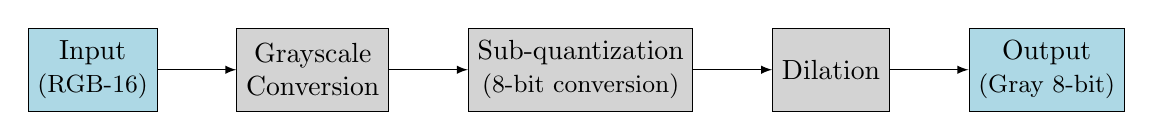
\begin{tikzpicture}
  \tikzset{
    Box/.style={draw, align=center, minimum height=30pt},
    ImageBox/.style={Box, fill=LightBlue},
    AlgoBox/.style={Box, fill=LightGrey}
  };


  \node[ImageBox] (A0) []            {Input\\ \small (RGB-16)};
  \node[AlgoBox]  (A1) [right=of A0] {Grayscale\\Conversion};
  \node[AlgoBox]  (A2) [right=of A1] {Sub-quantization\\ \small (8-bit conversion)};
  \node[AlgoBox]  (A3) [right=of A2] {Dilation};
  \node[ImageBox] (A4) [right=of A3] {Output\\ \small (Gray 8-bit)};

  \draw[-latex] (A0) -- (A1);
  \draw[-latex] (A1) -- (A2);
  \draw[-latex] (A2) -- (A3);
  \draw[-latex] (A3) -- (A4);
\end{tikzpicture}
\end{document}